\documentclass[11pt]{jarticle}
\setlength{\textheight}{43\baselineskip}
\addtolength{\textheight}{\topskip}
\setlength{\textheight}{21\footskip}
\setlength{\textwidth}{42zw}
\setlength{\hoffset}{-5zw}
\usepackage{amsmath,amssymb,bm}
%
\usepackage{fancyhdr} %ヘッダー
\pagestyle{fancy}
\rhead{物理数学 \ 2016.04.18}
\renewcommand{\headrulewidth}{0pt} %ヘッダーラインを打ち出さない
%
\def \bun#1#2{\left(\frac{#1}{#2}\right)} %括弧付き分数マクロ
\def \vec#1{\mbox{\boldmath $#1$}} %ベクトルマクロ
\def \rot{\nabla \times} %ローテーション
\def \div{\nabla \cdot} %ダイバージェンス
\def \intt{\int\!\!\!\int} %2重積分
\def \intf#1#2#3#4{\int_{#1}^{#2}\!\!\!\int_{#3}^{#4}} %2重積分範囲付き
\def \inttt{\int\!\!\!\int\!\!\!\int} %3重積分
\def \intff#1#2#3#4#5#6{\int_{#1}^{#2}\!\!\!\int_{#3}^{#4}\!\!\!\int_{#5}^{#6}} %3重積分範囲付き
%
\usepackage{graphicx}
%%------------------------------%%
\begin{document}
\begin{center}
{\Large
演習問題その4小テスト}\\
\ \\
\underline{学籍番号:          }, 
\underline{氏名:            }
\end{center}
\begin{enumerate}
%%-----(問題開始)-----%%
\item[1.]
デカルト座標系で,$\vec{a}=y \vec{e}_x - x \vec{e}_y + \left(x^2+y^2 \right) \vec{e}_z$
と表示されるベクトル$\vec{a}$を,図のような円柱座標系$(\rho,\phi,z)$で表せ.
\begin{figure}[h]
 \begin{center}
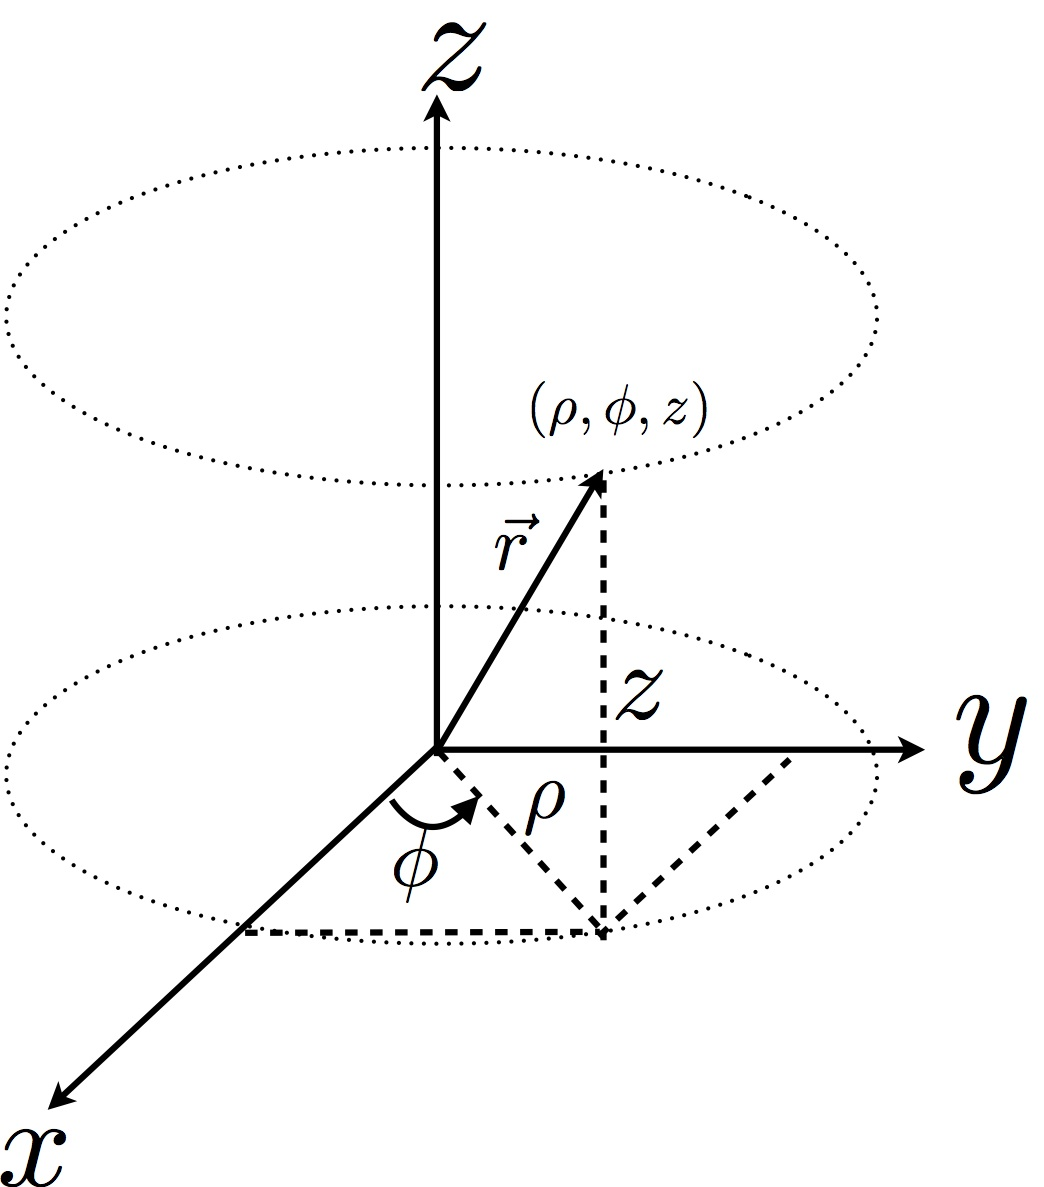
\includegraphics[keepaspectratio,width=50mm]{cylinder.eps}\caption{円柱座標系}
\end{center}
\label{fig:1}
\end{figure}

\newpage
\begin{center}
\underline{学籍番号:          }, 
\underline{氏名:            }
\end{center}

\item[2.]
図のように点A,B,Cをそれぞれ$\left(x, y, z \right)=\left(1, 0, 0 \right)$,$\left(0, 1, 0 \right)$,$\left(0, 0, 1 \right)$とする.
このときベクトル$\vec a=z \bm{e}_{x}+x \bm{e}_{y}+y \bm{e}_{z}$を点A$\rightarrow$
点B$\rightarrow$点C$\rightarrow$点Aの経路で線積分せよ.
\begin{figure}[h]
\begin{center}
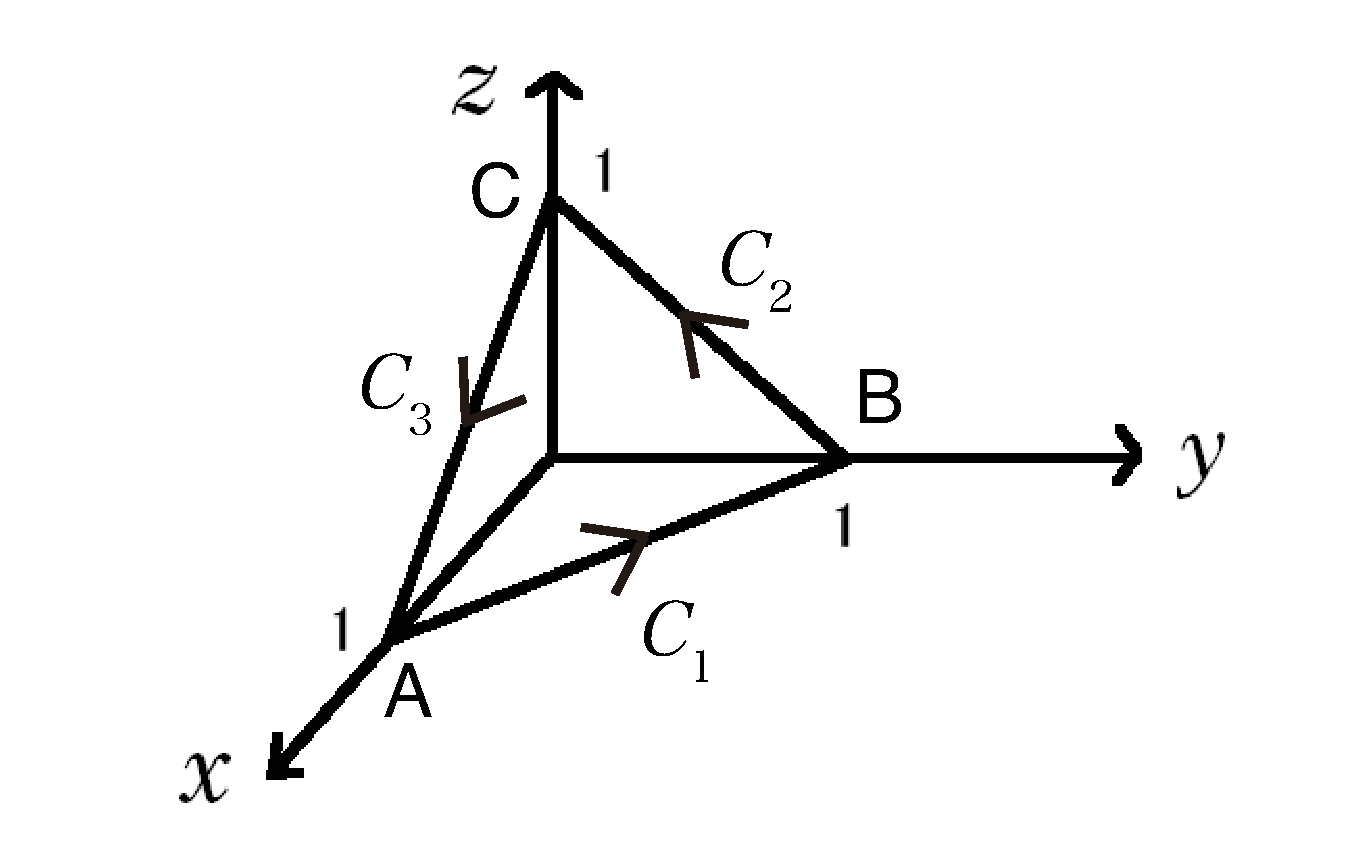
\includegraphics[width=.4\textwidth
%,bb=19 19 400 340
]{3men.eps}
\label{b}
\end{center}
\end{figure}
%%-----(問題終了)-----%%
\end{enumerate}


\newpage
%%------------------------------%%
%%-----(   解答ここから   )-----%%
\begin{center}
{\Large
演習問題その4小テスト 解答例}\\
\end{center}
\begin{enumerate}
\item[1.]
デカルト座標系で,$\vec{a}=y \vec{e}_x - x \vec{e}_y + \left(x^2+y^2 \right) \vec{e}_z$
と表示されるベクトル$\vec{a}$を,図のような円柱座標系$(\rho,\phi,z)$で表せ.
\begin{figure}[h]
 \begin{center}
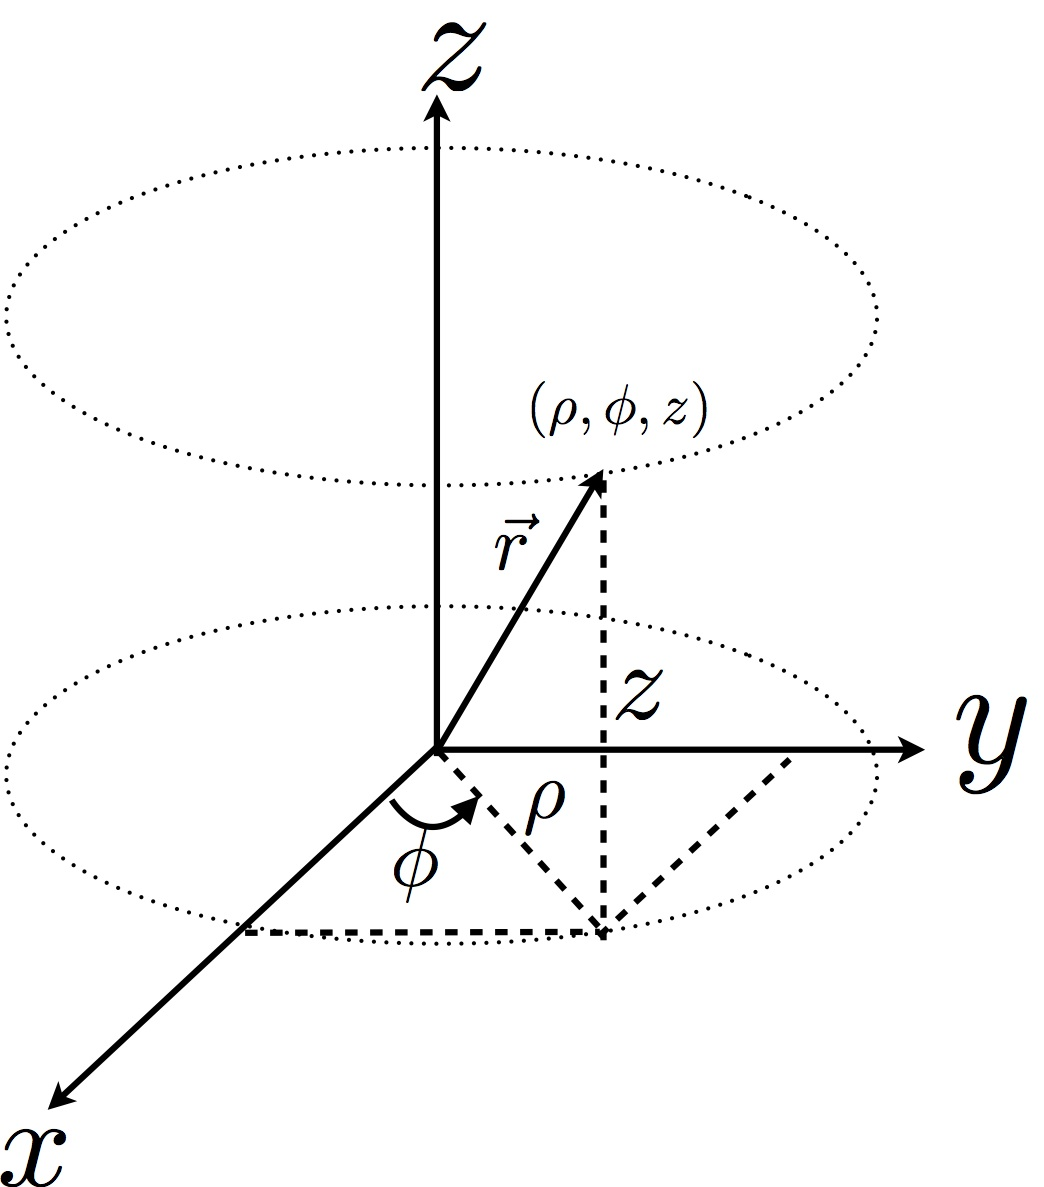
\includegraphics[keepaspectratio,width=50mm]{cylinder.eps}\caption{円柱座標系}
\end{center}
\label{fig:1}
\end{figure}
\\
(解答例)\\
$x=\rho\cos\phi,\ y=\rho\sin\phi$であり,さらに
\begin{eqnarray*}
{\Vec e}_{\it x}&=&\cos\phi{\Vec e}_{\rho}-\sin\phi{\Vec e}_{\phi} \\
{\Vec e}_{\it y}&=&\sin\phi{\Vec e}_{\rho}+\cos\phi{\Vec e}_{\phi} \\
{\Vec e}_{\it z}&=&{\Vec e}_{\it z}
\end{eqnarray*}
であるので,代入して整理すると,
\begin{eqnarray*}
{\Vec a}= -\rho \vec{e}_{\phi}+ \rho^2 \vec{e}_z.
\end{eqnarray*}


\newpage
\item[2.]
図のように点A,B,Cをそれぞれ$\left(x, y, z \right)=\left(1, 0, 0 \right)$,$\left(0, 1, 0 \right)$,$\left(0, 0, 1 \right)$とする.
このときベクトル$\vec a=z \bm{e}_{x}+x \bm{e}_{y}+y \bm{e}_{z}$を点A$\rightarrow$
点B$\rightarrow$点C$\rightarrow$点Aの経路で線積分せよ.
\begin{figure}[h]
\begin{center}
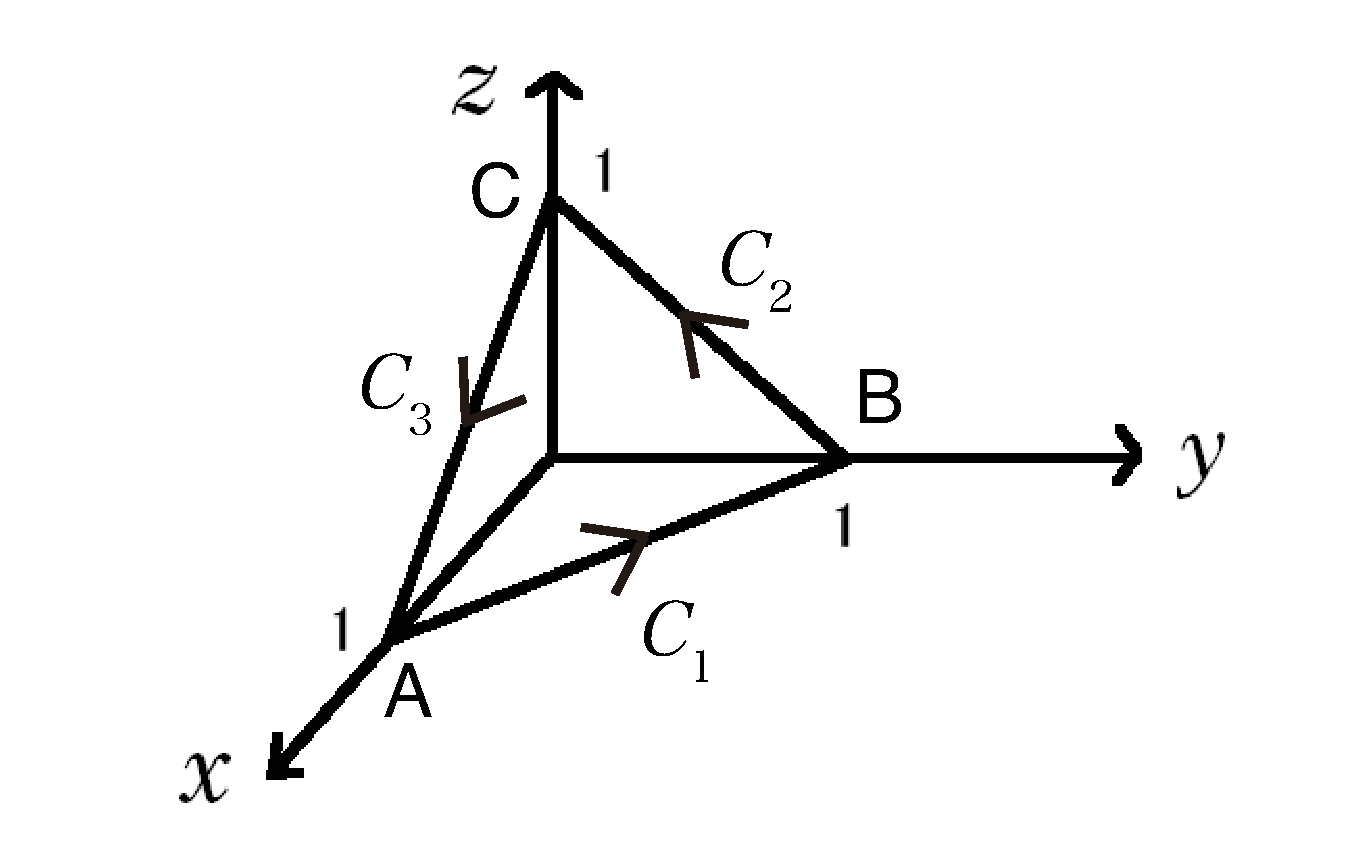
\includegraphics[width=.4\textwidth
%,bb=19 19 400 340
]{3men.eps}
\label{b}
\end{center}
\end{figure}
\\
(解答例)\\
まず経路$C_1$について考える。\\
経路$C_1$上の位置ベクトルは,媒介変数$t \ \left(0 \le t \le 1 \right)$を用いて$\bm{r}=(1-t)\bm{e}_{x}+t \bm{e}_{y}$と書けるから,
$\mathrm{d} \bm{r}=(-\bm{e}_{x}+\bm{e}_{y})\mathrm{d}t$.$z=0, x=1-t, y=t$に注意して,経路$C_1$上での線積分を計算すると,
%
\begin{eqnarray*}
\label{a}
\int_{C_1} \bm{a}\cdot \mathrm{d}\bm{r}&=&
\int_0^1 \left(x \bm{e}_y + y \bm{e}_z \right) \cdot \left(-\bm{e}_{x}+\bm{e}_{y} \right)\mathrm{d}t \\[8pt]
&=& \int^1_0 (1-t) \mathrm{d}t = \frac{1}{2}.
\end{eqnarray*}
経路$C_2, C_3$については$x=1-t, y=t, z=0$を$x=0, y=1-t, z=t$あるいは$x=t, y=0, z=1-t$に変えることで$C_1$の場合と全く同様に計算できるので,
\begin{eqnarray*}
\label{a}
\oint_C \bm{a} \cdot \mathrm{d}\bm{r}=3\int_{C_1} \bm{a}\cdot \mathrm{d}\bm{r}=\frac{3}{2}
\end{eqnarray*}

%%-----(解答終了)-----%%
\end{enumerate}
\end{document}
